\documentclass[a4paper, 12pt]{report}

\usepackage[utf8]{inputenc}
\usepackage[T1]{fontenc}
\usepackage[francais]{babel}
\usepackage{graphicx}
\usepackage{amsthm}
\usepackage{amsfonts}
\usepackage{amssymb}
\usepackage{amsmath}
\usepackage{textcomp}
\usepackage{hyperref}
\usepackage{stmaryrd} %llbracket and rrbracket
\usepackage{ dsfont }


%Liens hypertexte
\hypersetup{
    colorlinks,
    citecolor=black,
    filecolor=black,
    linkcolor=blue,
    urlcolor=black
}

%Découpe des mots
\hyphenation{}

%Alinéa
%\setlength{\parindent}{2 cm}


\setcounter{tocdepth}{1}
\setcounter{secnumdepth}{1}

%Paramètre de la page
\headheight=0mm
\topmargin=-10mm
\oddsidemargin=-1cm
\evensidemargin=-1cm
\textwidth=18cm
\textheight=25.5cm
\parindent=0mm



%Création du Titre
\title{ \bf Fractales et dimension de Hausdorff}
\author{Mechineau Alexandre}

\makeindex




\begin{document}
	%Creation du paragraphe définition
	\newtheorem{definition}{Définition}
	\newtheorem{prop}{Proposition}
	\newtheorem{theorem}{Théorème}
	\newtheorem*{remark*}{Remarque}
	\newtheorem{lemma}{Lemme}
	
	
	\maketitle
	
	\begin{abstract}
		Je vais définir ce qu'est un ensemble auto-similaire puis chercher à caractériser sa dimension dans l'espace. 
	\end{abstract}
	
	\tableofcontents
	
	\chapter{\bf Introduction}
	
	\chapter{\bf Ensemble auto-similaire et fractales}
		\section{Rappel}
			Dans un premier temps je vais définir ce qu'est un espace métrique. Puis, je rappellerais ce qu'est les notions d'espaces complets et d'espace compact. Enfin, je rappellerai la notion d'application contractante et énoncerai le Théorème du points fixe de Banach(Picard).
			
			\begin{definition}
				On appelle $(E,d)$ un \textbf{espace métrique} si $E$ est un ensemble et $d$ une distance sur E.
				
				On appelle distance sur un ensemble $E$ une application:
				\begin{equation*}
					d:E^2\longrightarrow \mathds{R}
				\end{equation*}
			Tel que pour tout $x$,$y$,$z$ $\in E$:
				\begin{enumerate}\itemsep2pt
					\item $d(x,y)=d(y,x)$
					\item $d(x,y)=0 \Longrightarrow x=y$
					\item $d(x,z) \leq d(x,y)+d(y,z)$
				\end{enumerate}
			\end{definition}
			
			\begin{definition}
				Un espace métrique $(E,d)$ est dit \textbf{complet} si toute suite de Cauchy de $E$ admette une limite dans $E$.
				\label{espMetriqueDef}
			\end{definition}
			
			\begin{definition}
				Un espace métrique $(E,d)$ est dit \textbf{pré-compact} si pour tout $\varepsilon >0$, on peut peut recouvrir $E$ par un nombre fini de boule ouverte de rayon $\varepsilon$.
			\end{definition}
			
			\begin{definition}
				Un espace métrique $(E,d)$ est dit \textbf{compact} 
			\end{definition}
			
			\begin{prop}
				Un espace métrique est \textbf{compact} si et seulement si il est \textbf{complet} et \textbf{pré-compact}.
			\end{prop}
			
			\begin{definition}
				Soit $(E,d)$ un espace métrique et $K$ un sous-espace de $E$.
				\begin{itemize}
					\item Un ensemble fini $A$ est appelé \textbf{r-recouvrement} de $K$ si et seulement si:
					\begin{equation*}
						\cup_{x\in A} \mathcal{B}_r(x)\supseteq K
					\end{equation*}
					\item $K$ est dit \textbf{pré-compact} si et seulement si il existe un r-recouvrement de $K$ pour tout $r>0$.

				\end{itemize}

			\end{definition}

			\hspace{.7 cm}
			J'ai donc définit ce qu'est un espace métrique et je l'ai décrit. Je peux donc définir ce qu'es une application contractante.
			\begin{definition}
				Une application $f$ d'un espace métrique $(E,d)$ est dite \textbf{contractante} si:
				\begin{equation}
					\exists k\in\mathds{R}^+, k<1 \mid \forall x,y\in E, d(f(x),f(y))\leqslant k\times d(x,y)
					\label{Pcontractante}
				\end{equation}
			\end{definition}
			
			\begin{remark*}
				Une application est contractante  par rapport à une distance donnée!
			\end{remark*}

			\hspace{.7 cm}Comme nous le verrons plus tard, cette propriété de contraction est la clé pour pouvoir définir ce que sont les fractales définies par IFS. 
			\begin{prop}
				\begin{itemize}
					\item Les homothéties de rapport inférieur à 1 sont des applications contractantes.
					\item Les similitudes de rapport inférieur à 1 sont des applications contractantes.
				\end{itemize}
			\end{prop}
			\hspace{.7 cm}Ces deux propriétés sont essentielles par la suite. En effet, l'ensemble des fractales qui seront étudiées sont définies par de telle applications.
			
			\begin{theorem}[\textbf{Théorème du points fixe de Banach(Picard)}]
				\label{ThmPtFixe}
				Soit $(E,d)$, un espace métrique complet et $f$ une application k-contractante de $E$ dans $E$. Alors, il existe un unique points fixe $x^*$ de $f$:
				\begin{equation*}
					x^*\in E\mid x^*=f(x^*)
				\end{equation*}
				De plus, pour toute suite d'éléments $(x_n)_{n\in\mathds{N}}$ de $E$ vérifiant la récurrence :
				\begin{equation*}
					x_{n+1}=f(x_n)
				\end{equation*}
				On a,
				\begin{equation}
					d(x_n,x^*)\leq \frac{k^n}{1-k} d(x_0,x_1)
				\end{equation}
				Donc, la suite $(x_n)$ converge vers $x^*$.
				On note aussi, $\forall a\in E,(f^n(a))_{n\geq 0}\longrightarrow x^*$ si $x^*$est un points fixe.
			\end{theorem}

			\begin{proof}
				Soit $(X,d)$ un espace complet.\\
				Soit $f$ une application k-contractante de $E$ dans $E$.\\
				On pose $m,n\in\mathds{N}\mid m>n,a\in E$\\
				\begin{align*}
					d(f^n(a),f^m(a))&\leq d(f^n(a),f^{n+1}(a))+\ldots+d(f^{m-1}(a),f^m(a))  \tag{Inégalité triangulaire}\\
									&\leq (k^n+\ldots+k^{m-1})d(a,f(a)) \tag*{\eqref{Pcontractante}}\\
									&\leq \frac{k^n}{1-k}d(a,f(a))
				\end{align*}
				La série $(f^n(a))_{n\geq 0}$ est de Cauchy. En effet, elle converge vers $x^*$ quand $n\longrightarrow\infty$.
				Or $(E,d)$ est un espace complet donc $x^*\in E$ (Définition \ref{espMetriqueDef}).
				On a alors $x^*=f(x^*)$\\
				\textbf{Unicité du point fixe :}
				\begin{align*}
					f(x)=x \textrm{ et } f(y)=y\\
					&d(x,y) = d(f(x),f(y)) \leq k\times d(x,y)\\
					&d(x,y) \leq k\times d(x,y)
					&\Rightarrow d(x,y)=0\Rightarrow x=y \tag{Unicité}
				\end{align*}
			\end{proof}



		\section{Ensemble auto-similaire}
		
			\begin{theorem}[Unicité et existence des ensembles auto-similaires]
			\label{thmPrincipale}
				Soit $(E,d)$ un espace complet.\\
				$\forall i \in \llbracket 1,N \rrbracket, f_i:E \longrightarrow E$ est une application contractante, par rapport à la distance $d$.\\
				Il existe, alors un compact $K\subset E$, tel que:
				\begin{equation*}
					K=\cup^N_{i=1}f_i(K)
				\end{equation*}
				$K$ est appelé un \textbf{ensemble auto-similaire} défini par :
				\begin{equation*}
					\{f_1,\ldots\,f_N\}
				\end{equation*}
			\end{theorem}
		
			\begin{remark*}
			\hyperref[ThmPtFixe]{Le Théorème du point fixe de Banach} est un cas particulier de ce théorème avec $N=1$.
			\end{remark*}
		
			Pour simplifier, on pose :
			\begin{equation*}
				F(A)=\cup^N_{i=1}f_i(A)
			\end{equation*}
			De plus, on introduit l'ensemble suivant pour tout $(E,d)$ espace complet:
			\begin{equation*}
				\mathcal{C}(E) : \{A|A\subseteq E, A\textrm{ est un compacte non vide de }E\}
			\end{equation*}
			
			\hspace{.7 cm}On va maintenant définir une métrique $\delta$ sur $\mathcal{C}(E)$ nommée \textit{mesure de Hausdorff} sur $\mathcal{C}(E)$.
			\begin{prop}
				\label{mesHauss}
				Pour $A,B\in\mathcal{C}(E),$ et $(E,d)$ un espace métrique\\
				On définit $\delta(A,B)=\inf\{r>0\mid U_r(A)\supseteq B, U_r(B)\supseteq A\}$\\
				On pose, pour $r>0$ fixé, $U_r(A)=\{x\in E\mid d(x,y)\leq r,y\in A\}$\\
				$\delta$ est alors une distance sur $\mathcal{C}(E)$.\\$(E,d)$
				De plus, si $(E,d)$ est complet alors $(\mathcal{C}(E),\delta)$ est complet.
			\end{prop}
			\begin{remark*}
				La mesure $\delta$ dépends de la mesure $d$ de l'ensemble $E$ comme nous pouvons le voir dans la définition. 
			\end{remark*}

			
			\hspace{.7 cm}Nous pouvons alors montré que $\delta$ est une distance. Pour ce faire nous allons 
			\begin{proof}
				Soit un compact $A\subseteq X$,\\
				On va montrer que $F$ admet un point fixe.\\
				Pour cela, on pose \\
				\textbf{Preuve que la mesure de HAUSDORFF est bien une mesure!!!!!!!!!!!}
			\end{proof}
			
			\begin{theorem}
			\label{ThmConverge}
				Soit $(E,d)$ un espace métrique complet.\\
				Soit 
				\begin{align*}
					F:&\mathcal{C}(E)\longrightarrow \mathcal{C}(E)\\
					&A\longmapsto F(A)=\cup^N_{i=1}f_i(A)
				\end{align*}
				et $f_i:X \longrightarrow X, i\in\llbracket 1,N\rrbracket$\\
				Alors $F$ admet un unique points fixe K. De plus, $\forall A\in\mathcal{C}(E), F^n(A)\longrightarrow K$ quand ${n\to\infty}$ par rapport à la mesure de Hausdorff.
			\end{theorem}

			\begin{lemma}
				\label{lemme118}
				$\forall A_1,A_2,B_1,B_2\in\mathcal{C}(E),$ on a :
				\begin{equation}
					\label{HaussMajUnion}
					\delta(A_1\cup A_2 , B_1\cup B_2)\leq \max(\delta(A_1,B_1), \delta(A_2,B_2))
				\end{equation}
			\end{lemma}
		
			\begin{proof}
				Si r>$\max(\delta(A_1,B_1), \delta(A_2,B_2))$, alors $U_r(A_1)\supseteq B_1$ et $U_r(A_2)\supseteq B_2$. Par conséquent, $U_r(A_1\cup A_2)\supseteq B_1\cup B_2$.\\
				De même, $U_r(B_1)\supseteq A_1$ et $U_r(B_2)\supseteq A_2\Longrightarrow U_r(B_1\cup B_2)\supseteq A_1\cup A_2$.\\
				On a donc $r\geq \max(\delta(A_1,B_1), \delta(A_2,B_2)) $ (\ref{HaussMajUnion})
			\end{proof}

			\begin{lemma}
			\label{lemme119}
				Si $f$ est une application $k$-contractante défini de $\mathcal{C}(E)$ dans $\mathcal{C}(E)$, alors :
				\begin{equation}
					\delta(f(A),f(B))\leq k\times \delta(A,B),\forall A,B\in\mathcal{C}(E)
				\end{equation}
			\end{lemma}
			
			\begin{proof}
				On sait qu'il existe $s\geq\delta(A,B)$ tel que:
				\begin{equation*}
					U_s(A)\supseteq B \textrm{ et } U_s(B)\supseteq A,  U_{sk}(f(A))\supseteq f(U_s(A))\supseteq f(B)					
				\end{equation*}
				\begin{equation*}
					U_s(B)\supseteq A \textrm{ et } U_s(A)\supseteq B,  U_{sk}(f(B))\supseteq f(U_s(B))\supseteq f(A)
				\end{equation*}
				On a donc montré que $\delta(f(A),f(B))\leq k*s\leq k*\delta(A,B)$

			\end{proof}

			\begin{proof}[Preuve du théorème]
				On applique le Lemme \ref{lemme118}, on obtient alors:
				\begin{align*}
					\delta(F(A),F(B))	&=\delta(\bigcup_{i=1}^N f_i(A),\bigcup_{i=1}^N f_i(B))\\
										&\leq\max_{1\leq i\leq N}\{\delta(f_i(A),f_i(B))\}
				\end{align*}
				D'après le lemme \ref{lemme119} on a:
				\begin{align*}
					\delta(f_i(A),f_i(B))\leq r_i\times\delta(A,B)
				\end{align*}
				On a alors,
				\begin{align*}
					\delta(F(A),F(B))	&\leq\max_{1\leq i\leq N}\{r_i\times\delta(A,B)\}\\
										&\leq \left\lgroup\max_{1\leq i\leq N}\{r_i\}\right\rgroup\times\delta(A,B)
				\end{align*}
				$F$ est donc une application contractante par rapport à la distance de Hausdorff. D'après la proposition \ref{mesHauss}, on sait que $\mathcal{C}(E)$ est complet donc d'après \hyperref[ThmPtFixe]{Le Théorème du point fixe}, $F$ admet un point fixe.
			\end{proof}
		\section{Ensemble auto-similaire et fractale}
			Un ensemble auto-similaire est la traduction du mot anglais ``self-similarity''. Ce mot représente le fait qu'un objet présente des similarités peu importe l'échelle à laquelle il est regardée. On va étudier les fractales définies par un système de fonction contractante, on sera donc dans le cas des ensembles auto-similaires. On choisit $E=\mathds{R}^2$ et on lui associe la distance usuelle. L'espace métrique défini est complet. On pourra donc utiliser l'ensemble des théorèmes et propositions précédente. Les fonctions qui définirons notre fractale seront des similitudes contractante. Nous munirons notre fractale d'un sous-compact de $E=\mathds{R}^2$ qui sera le plus adapté à la fractale même si comme nous pourrons le voir cela n'a pas d'importance sur le papier. 
			\begin{definition}
				Une \textbf{similitude} est une application de $E$ dans $E$ qui multiplie les distances par un rapport $k$ constant.
			\end{definition}
			\begin{remark*}
				On peut représenter une similitude comme la composée d'une homothétie, d'une rotation(ou symétrie) et d'une translation.
			\end{remark*}
			\begin{prop}
				Soit S une similitude, soit $k$ son rapport,$\theta$ son angle de rotation et $T$ un vecteur de translation. On peut écrire S sous la forme suivante:
				\begin{align*}
					S(X)=k\times M(\theta)\times X+T
				\end{align*}
				On pose M étant une rotation directe ou indirecte:
				\begin{align*}
					M(\theta)\in\Bigg\{
					\begin{pmatrix}
						\cos(\theta) & -\sin(\theta) \\
						\sin(\theta) & cos(\theta) 
					\end{pmatrix}
					,
					\begin{pmatrix}
						\cos(\theta) & \sin(\theta) \\
						\sin(\theta) & -cos(\theta) 
					\end{pmatrix}
					\Bigg\}
				\end{align*}
			\end{prop}

			\begin{definition}
				Une fractale défini par un ensemble de similitude contractante est appelé \textbf{IFS} (Iterated function system). 
			\end{definition}
			
			\hspace{.7 cm}On remarque qu'une fractale défini par IFS est un ensemble auto-similaire. On sait alors grâce au théorème \ref{thmPrincipale} qu'il existe un unique points fixe(Ensemble). De plus, on sait grâce au théorème \ref{ThmConverge} que pour tout compact de $\mathds{R}^2$ le système converge vers le même ensemble.

	\chapter{\bf Dimension des ensembles auto-similaires}
		\section{Dimension de Hausdorff}
	
	\chapter{IFS et informatique}
			
			On sait que l'on peut décrire une fractale IFS par un ensemble de similitude et un compact. Le choix du compact a seulement de l'importance pour avoir un résultat "correct" le plus rapidement. Pour calculer le premier pas de la fractale on applique chaque similitude sur l'ensemble de départ. On obtient, alors, une liste d'ensemble. Pour la deuxième étape, on utilise la liste d'ensemble précédemment obtenue sur lequel on applique chaque similitude.
			
			
			\vspace{.2 cm}\hspace{.7 cm}
			On utilise comme compact de base un segment, il nous permet de décrire chaque forme nécessaire aux fractales IFS que l'on représentera. On a alors à chaque étape une liste de segment défini par deux points. Cette liste a une taille qui suit une croissance exponentielle. Mais à chaque itération on se rapproche du points fixe. En pratique, à partir de cinq itérations le résultat est correct à l'échelle normale.
			
			\vspace{.2 cm}\hspace{.7 cm}
			D'un point de vue algorithmique, j'ai crée un objet application qui me permet de représenter l'ensemble des applications nécessaire de $\mathds{R}^2$. Puis j'ai créé des objets représentant des applications plus spécifique, mais dépendant de Application, comme Rotation, Homothétie, ...
			
			\vspace{.2 cm}\hspace{.7 cm}
			J'ai aussi créé un objet Forme décrivant par un ensemble de points un polygone de $\mathds{R}^2$. Cette objet forme représente un compact, c'est en effet l'union de plusieurs segments qui sont compact.
			
			\vspace{.2 cm}\hspace{.7 cm}
			J'ai écrit un dernier objet Fractale me permettant de définir une fractale IFS comme un ensemble d'Applications et un ensemble de Forme.
			
			\vspace{.2 cm}\hspace{.7 cm}
			L'objet Application permet d'appliquer l'application définie sur un ensemble de forme. Ce qui revient à calculer l'image de chaque extrémité des segments définissant l'objet Forme.
	
			\vspace{.2 cm}\hspace{.7 cm}
			En appliquant l'ensemble des Applications $n$ fois sur la Forme initiale on obtient la n-ème étape de la construction de la fractale. Il ne reste plus qu'à afficher chaque étape à l'écran.
	
	
	
	\chapter{\bf Exemple de fractale}
		\section{Notation}
		On note $SD$ les similitudes directes du plan.\newline
		On note $SI$ les similitudes indirectes du plan.\newline
		$M_d(\theta)$ est la matrice de rotation directe du plan d'angle $\theta$.\newline
		$M_i(\theta)$ est la matrice de rotation indirecte du plan d'angle $\theta$.\newline
		$H$ est une homothétie de rapport $k$.
		$x$ est un élément d'un compact de $\mathds{R}$ ou du plan.\newline
		$k$ est le rapport d'une similitude.\newline
		$\theta$ est l'angle d'une similitude.\newline
		$T$ est un vecteur représentant une translation.\newline
		
		\begin{align*}
			M_D(\theta)&=\left(	\begin{array}{ccc}
							\cos(\theta) &  -\sin(\theta) \\
							\sin(\theta) &  \cos(\theta)  \\
						\end{array} \right)\\
			M_I(\theta)&=\left(	\begin{array}{ccc}
							\cos(\theta) &  \sin(\theta) \\
							\sin(\theta) &  -\cos(\theta)  \\
						\end{array} \right)\\
			SD(x)&=k\times M_D(\theta)\times x + T\\
			SI(x)&=k\times M_I(\theta)\times x + T\\
			H(x)&=k\times M_D(0)\times x +T=k\times x+T
		\end{align*}
		\hspace{.7 cm} De même on peut représenter les similitudes grâce au complexe. Cela sera particulièrement utile pour la fractale de Hata.
		\begin{align*}
			&z\in\mathds{C} \textrm{ et } a\in\mathds{C}^*,b\in\mathds{C}\textrm{ fixés},\\
			&SD(z)=az+b\\
			&k=\lvert a\rvert
			&\theta
		\end{align*}


		\newpage
		\section{Cantor}
			\subsection{Définition}
				Pour l'ensemble de Cantor on part du segment $[0;1]$ que l'on contracte de $1/3$ à droite et gauche.
				On a donc deux homothéties de rapport 1/3 de centre 0 et 1. L'ensemble de départ et d'arrivé pour chaque application est $\mathds{R}.$ 
				\begin{align*}
					&H_1:x\mapsto 1/3\times x\\
					&H_2:x\mapsto 1/3\times x+2/3
				\end{align*}
			\subsection{Dimension}
				Pour calculer la dimension de Hausdorff de l'ensemble de Cantor on utilise le théorème (REFERENCE). On a alors,
				\begin{align*}
					\left(\frac{1}{3}\right)^d+\left(\frac{1}{3}\right)^d	&=1\\
											  2\left(\frac{1}{3}\right)^d	&=1\\
											   \left(\frac{1}{3}\right)^d	&=\frac{1}{2}\\
						\exp\left(d\times\ln\left(\frac{1}{3}\right)\right)	&=\frac{1}{2} \tag{Passage à la forme exponentielle}\\
										d\times\ln\left(\frac{1}{3}\right)	&=\ln\left(\frac{1}{2}\right)\\
																		d	&=\frac{\ln\left(\frac{1}{2}\right)}{\ln\left(\frac{1}{3}\right)}\\
																		d	&=\frac{\ln(1)-\ln(2)}{\ln(1)-\ln(2)}\\
																		d	&=\frac{\ln(2)}{\ln(3)} \tag{$\ln(1)$=0}\\
																		d	&\approx 0.6309
				\end{align*}
				On a donc calculer la dimension de Hausdorff de l'ensemble de Cantor.
				
				
				On se base sur ce calcule pour le reste des fractales.
				
				
				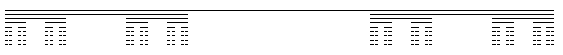
\includegraphics[scale=0.8]{Images/cantor}
		\newpage
		\section{Courbe de Koch}
			\subsection{Définition}
				Pour la courbe de Koch on part aussi du segment $[0;1]$. On définit quatre similitude directe du plan.
				\begin{align*}
					&SD_1:x\mapsto 1/3\times x\\
					&SD_2:x\mapsto 1/3\times M_d(\pi/3)\times x+\left(	\begin{array}{ccc}
															1/3\\
															0\\
														\end{array}\right)\\
					&SD_3:x\mapsto 1/3\times M_d(-\pi/3)\times x+\left(	\begin{array}{ccc}
															1/2\\
															\sqrt{3}/6\\
														\end{array}\right)\\
					&SD_4:x\mapsto 1/3\times x+\left(	\begin{array}{ccc}
															2/3\\
															0\\
														\end{array}\right)
				\end{align*}
			\subsection{Dimension}
				La courbe de Koch est constitué de quatre similitudes de rapport $1/3$. On a alors:
				\begin{align*}
					 4\left(\frac{1}{3}\right)^d	&=1\\
												d	&=\frac{\ln(4)}{\ln(3)}\\
												d	&\approx 1.2618
				\end{align*}
				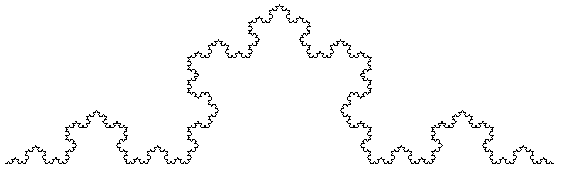
\includegraphics[scale=0.9]{Images/courbe}
			
		\newpage
		\section{Flocon de Koch} 
			\subsection{Définition}
				Le flocon de Koch est l'union de trois courbe de Koch. Elle est défini par sept similitudes et la forme de base est un triangle équilatéral de longueur $1$.
				\begin{align*}
					&SD_1:x\mapsto 1/3\times M_d(-2\pi/3)\times x+\left(	\begin{array}{ccc}
															1/6\\
															\sqrt{3}/6\\
														\end{array}\right)\\
					&SD_2:x\mapsto 1/3\times M_d(\pi/3)\times x+\left(	\begin{array}{ccc}
															1/6\\
															\sqrt{3}/6\\
														\end{array}\right)\\
					&SD_3:x\mapsto 1/3\times M_d(0)\times x+\left(	\begin{array}{ccc}
															1/3\\
															\sqrt{3}/3\\
														\end{array}\right)\\
					&SD_4:x\mapsto 1/3\times M_d(-\pi/3)\times x+\left(	\begin{array}{ccc}
															2/3\\
															\sqrt{3}/3\\
														\end{array}\right)\\
					&SD_5:x\mapsto 1/\sqrt{3}\times M_d(\pi/6)\times x+\left(	\begin{array}{ccc}
															1/3\\
															0\\
														\end{array}\right)\\
					&SD_6:x\mapsto 1/3\times M_d(\pi)\times x+\left(	\begin{array}{ccc}
															2/3\\
															0\\
														\end{array}\right)\\
					&SD_7:x\mapsto 1/3\times M_d(0)\times x+\left(	\begin{array}{ccc}
															1/3\\
															0\\
														\end{array}\right)
				\end{align*}
			\subsection{Dimension}
				Le flocon de Koch est constitué de six similitudes de rapport $1/3$ et une similitude de rapport $1/\sqrt{3}$. On a alors:
				\begin{align*}
					 6\left(\frac{1}{3}\right)^d+\left(\frac{1}{\sqrt{3}}\right)^d	&=1\\
																				d	&=2
				\end{align*}
				\begin{center}
					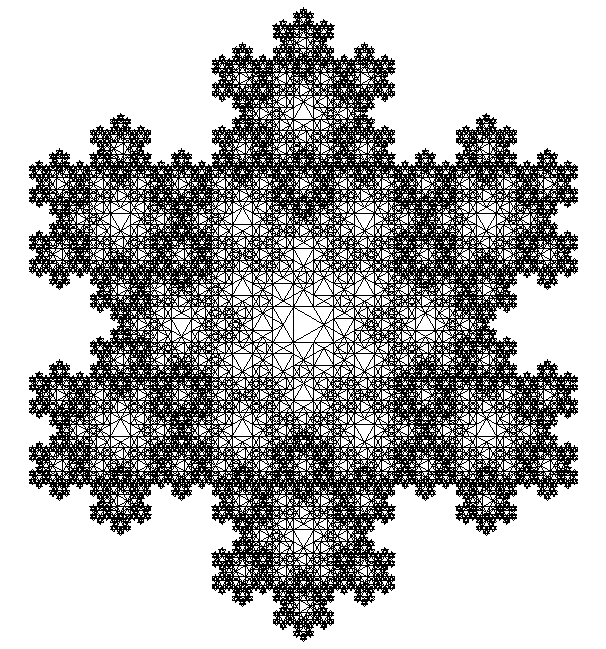
\includegraphics[scale=0.4]{Images/flocon}
				\end{center}
		\newpage
		\section{Triangle de Sierpiński}
			\subsection{Définition}
				Le triangle de Sierpiński est basé sur un triangle équilatéral de longueur 1. Il est constitué de trois homothétie de centre correspondant aux extrémités du triangle et de rapport $1/2$.
				\begin{align*}
					&H_1:x\mapsto 1/2\times x+\frac{1}{2}\left(	\begin{array}{ccc}
															0\\
															0\\
														\end{array}\right)\\
					&H_2:x\mapsto 1/2\times x+\frac{1}{2}\left(	\begin{array}{ccc}
															1\\
															0\\
														\end{array}\right)\\
					&H_3:x\mapsto 1/2\times x+\frac{1}{2}\left(	\begin{array}{ccc}
															1/2\\
															\sqrt{3/4}\\
														\end{array}\right)
				\end{align*}
			\subsection{Dimension}
				On a pour le triangle de Sierpiński:
				\begin{align*}
					 3\left(\frac{1}{2}\right)^d	&=1\\
												d	&=\frac{\ln(3)}{\ln(2)}\\
												d	&\approx 1.5849
				\end{align*}
				\begin{center}
					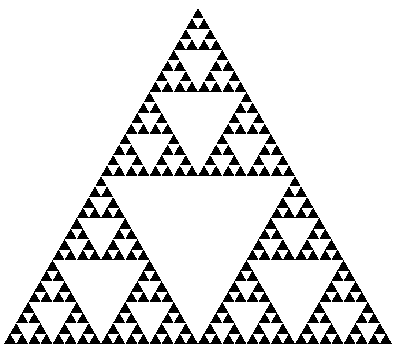
\includegraphics[scale=0.7]{Images/triangle}
				\end{center}
				
		\newpage
		\section{Tapis de Sierpiński}
			\subsection{Définition}
			Le tapis de Sierpiński est basé sur un carré, c'est a dire l'union de quatre segment. Il est constitué de 8 homothéties de rapport 1/3.
			\begin{align*}
				&H_1:x\mapsto 1/3\times x+\frac{1}{2}\left(	\begin{array}{ccc}
															0\\
															0\\
														\end{array}\right)\\
				&H_2:x\mapsto 1/3\times x+\frac{1}{2}\left(	\begin{array}{ccc}
																1\\
																0\\
															\end{array}\right)\\
				&H_3:x\mapsto 1/3\times x+\frac{1}{2}\left(	\begin{array}{ccc}
																1\\
																1\\
															\end{array}\right)\\
				&H_4:x\mapsto 1/3\times x+\frac{1}{2}\left(	\begin{array}{ccc}
																0\\
																1\\
															\end{array}\right)\\
				&H_5:x\mapsto 1/3\times x+\frac{1}{2}\left(	\begin{array}{ccc}
																1/2\\
																0\\
															\end{array}\right)\\
				&H_6:x\mapsto 1/3\times x+\frac{1}{2}\left(	\begin{array}{ccc}
																1\\
																1/2\\
															\end{array}\right)\\
				&H_7:x\mapsto 1/3\times x+\frac{1}{2}\left(	\begin{array}{ccc}
																1/2\\
																1\\
															\end{array}\right)\\
				&H_8:x\mapsto 1/3\times x+\frac{1}{2}\left(	\begin{array}{ccc}
																0\\
																1/2\\
															\end{array}\right)
			\end{align*}

			\subsection{Dimension}
				En appliquant, la formule une fois encore, on obtient:
				\begin{align*}
					 8\left(\frac{1}{3}\right)^d	&=1\\
												d	&=\frac{\ln(8)}{\ln(3)}\\
												d	&\approx 1.8928
				\end{align*}
				\begin{center}
					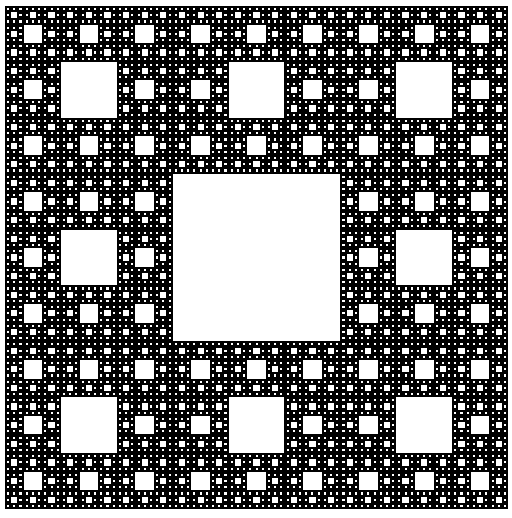
\includegraphics[scale=0.3]{Images/carpet}
				\end{center}
		\newpage
		\section{Hata's tree-like set}
			\subsection{Définition}
			Cette fractale représente de manière simpliste une branche d'arbre. Elle est défini à partir de deux formes le segment classique$[0;1]$ et un second segment ayant pour extrémité l'origine et un point du plan servant de paramètre. Elle est constitué deux similitudes indirectes. Au contraire des fractales précedente je vais me servir des complexes pour définir en partie la fractale.
			
			\subsection{Dimension}
			\begin{center}
				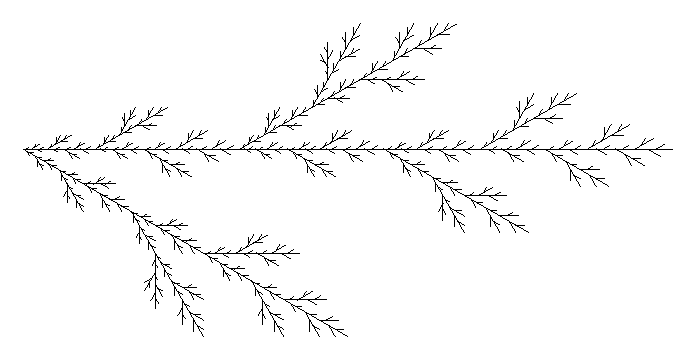
\includegraphics[scale=0.3]{Images/hata1}
				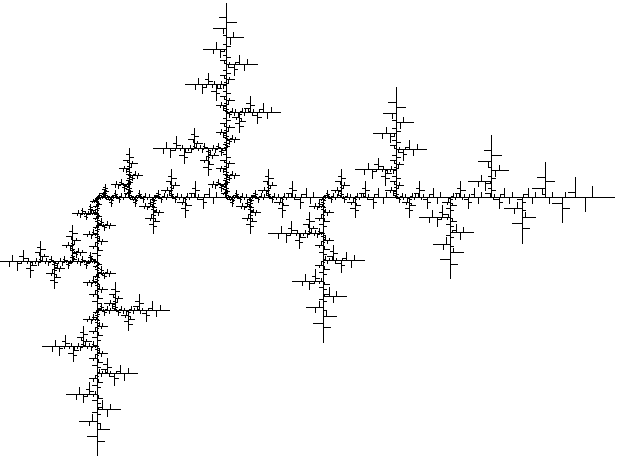
\includegraphics[scale=0.3]{Images/hata2}
			\end{center}

		\newpage
		\section{Courbe de Lévy}
			\subsection{Définition}
			La courbe de Lévy est définit à partir d'un segment. Elle est construite par deux similitudes directe de rapport $\frac{\sqrt{2}}{2}$.
			
			\subsection{Dimension}
				\begin{align*}
					 2\left(\frac{1}{\sqrt{2}}\right)^d	&=1\\
					 \left(\frac{1}{\sqrt{2}}\right)^d	&=\frac{1}{2}\\
													d	&=2
				\end{align*}
				\begin{center}
					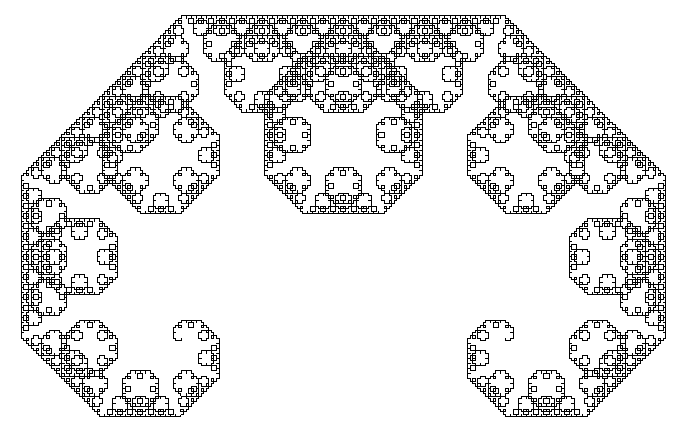
\includegraphics[scale=0.7]{Images/levy}
				\end{center}
		\newpage
		\section{PentaKun}
			\subsection{Définition}
			Le pentakun est basé comme son nom l'indique sur un pentagone. On définit donc cinq point.
			\begin{equation*}
				p_i=\left(\begin{array}{ccc}
							-\sin\left(\frac{2i\pi}{5}\right)\\
							\cos\left(\frac{2i\pi}{5}\right)\\
						\end{array}\right)
						,\forall i\in\textrm{\textlbrackdbl} 1,5\textrm{\textrbrackdbl}
			\end{equation*}
			On définit cinq homothétie qui vont réduire le pentagone dans chaque coins. Le rapport des homothéties est de $\frac{3-\sqrt{5}}{2}$.
			\begin{equation*}
				H_i=\frac{3-\sqrt{5}}{2}\times x+\frac{\sqrt{5}-1}{2}p_i,\forall i\in\textrm{\textlbrackdbl} 1,5\textrm{\textrbrackdbl}
			\end{equation*}
			\subsection{Dimension}
				\begin{align*}
					 5\left(\frac{3-\sqrt{5}}{2}\right)^d	&=1\\
					 \left(\frac{3-\sqrt{5}}{2}\right)^d	&=\frac{1}{5}\\
														d	&=\frac{-\ln(5)}{\ln(3-\sqrt{5})-\ln(2)}\\
														d	&\approx 1.6723
				\end{align*}
				\begin{center}
					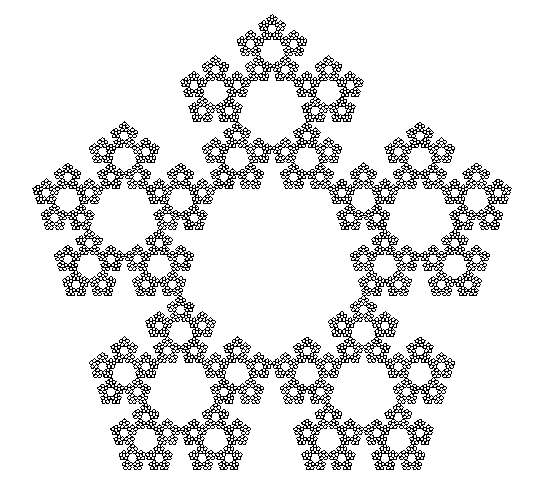
\includegraphics[scale=0.5]{Images/pentakun.png}
				\end{center}
				
http://ecademy.agnesscott.edu/~lriddle/ifs/kcurve/kcurve.htm

https://www.yumpu.com/es/document/view/14324138/analisis-armonico-en-fractales-universidad-de-colima/5
\end{document}

